%% Classification of compact hyperbolic Coxeter 6-polytopes with 10 facets.
%% Compile:  pdflatex paper && bibtex paper && pdflatex paper && pdflatex paper
\documentclass[11pt,reqno]{amsart}

\usepackage[T1]{fontenc}
\usepackage[utf8]{inputenc}
\usepackage{amsmath,amssymb,amsthm,mathtools}
\usepackage{booktabs}
\usepackage{longtable}
\usepackage{tikz}
\usepackage{array}
\usepackage{microtype}
\usepackage[margin=1.15in]{geometry}
\usepackage[colorlinks=true,linkcolor=blue!55!black,citecolor=blue!55!black,
            urlcolor=blue!55!black]{hyperref}

\usetikzlibrary{calc}

\theoremstyle{plain}
\newtheorem{theorem}{Theorem}[section]
\newtheorem{proposition}[theorem]{Proposition}
\newtheorem{lemma}[theorem]{Lemma}
\newtheorem{corollary}[theorem]{Corollary}
\theoremstyle{definition}
\newtheorem{definition}[theorem]{Definition}
\newtheorem{remark}[theorem]{Remark}
\newtheorem{assumption}[theorem]{Assumption}

\DeclareMathOperator{\conv}{conv}
\DeclareMathOperator{\rank}{rank}
\DeclareMathOperator{\sig}{sign}
\newcommand{\HH}{\mathbb{H}}
\newcommand{\RR}{\mathbb{R}}
\newcommand{\QQ}{\mathbb{Q}}
\newcommand{\ZZ}{\mathbb{Z}}
\newcommand{\Gr}{G}
\newcommand{\PP}{P_{6,10}}

\input{tables/summary_nums}

%% ---- Coxeter-diagram drawing conventions (matching Burcroff, Ma--Zheng) ----
%% single line = pi/3, double = pi/4, triple = pi/5, dashed = ultraparallel.
\newcommand{\cnode}[2]{\fill (#1) circle (2.4pt) node[#2] {}}
\newcommand{\esingle}[2]{\draw[line width=.5pt] (#1)--(#2);}
\newcommand{\edouble}[2]{%
  \draw[line width=1.9pt] (#1)--(#2);%
  \draw[line width=0.8pt,white] (#1)--(#2);}
\newcommand{\etriple}[2]{%
  \draw[line width=2.9pt] (#1)--(#2);%
  \draw[line width=1.9pt,white] (#1)--(#2);%
  \draw[line width=1.0pt] (#1)--(#2);%
  \draw[line width=0.35pt,white] (#1)--(#2);}
\newcommand{\edash}[2]{\draw[line width=.5pt,dashed] (#1)--(#2);}

\begin{document}
\title{The polytope $\PP$: diagram, Gram matrix, automorphisms,
and position relative to the Felikson--Tumarkin class}
\author{John Mcleod}
\address{Solvo.ai}
\maketitle

\noindent
This is a companion to \emph{Compact hyperbolic Coxeter $6$-polytopes with
$10$ facets, and the completion of the $d+4$ classification}. The polytope is not
new---it is drawn as Figure~5 of \cite{Burcroff2024}, attributed there to
Bugaenko \cite{Bugaenko1984}---so the paper states only that it is the unique
member of the family and does not redraw it. It is presented here for reference,
together with the automorphism computation behind ``exactly one up to isometry
and its position relative to the Felikson--Tumarkin class $\mathcal{P}$.
\bigskip

\section{The polytope}
Label the facets $1,\dots,10$. The Coxeter diagram of $\PP$ has ordinary edges
\[
\begin{aligned}
&(1,2,5),\ (2,3,3),\ (3,4,3),\ (4,5,3),\ (5,6,3),\\
&(9,10,5),\ (2,7,4),\ (2,8,4),\ (5,9,3),\ (6,10,5),
\end{aligned}
\]
written as $(i,j,m)$ for a dihedral angle $\pi/m$, all other intersecting pairs
being orthogonal, and dashed edges $\{6,7\},\{7,8\},\{8,9\}$ with weights
\[
w_{67}=w_{89}=\sqrt2\,(2+\sqrt5)=2\sqrt2+\sqrt{10}\approx 5.990705,
\qquad
w_{78}=17+8\sqrt5\approx 34.888544 .
\]
These satisfy $w_{78}=w_{67}^{\,2}-1$ exactly. The minimal polynomials are
$x^4-36x^2+4$ for $w_{67}=w_{89}$ and $x^2-34x-31$ for $w_{78}$, and both
weights lie in $\QQ(\sqrt2,\sqrt5)$, which is therefore the field generated by
the entries of the Gram matrix.

\begin{figure}[t]
\centering
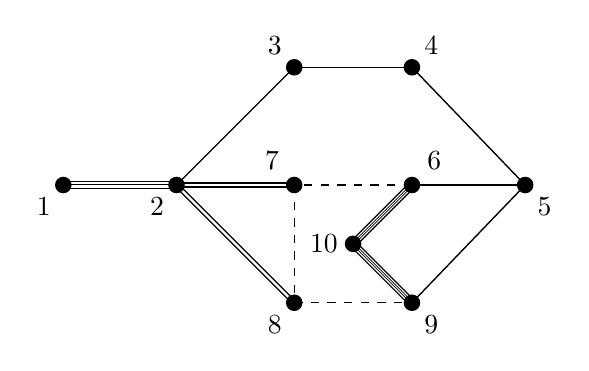
\begin{tikzpicture}[scale=1.15]
  \coordinate (n1)  at (0,0);
  \coordinate (n2)  at (1.25,0);
  \coordinate (n3)  at (2.55,1.3);
  \coordinate (n4)  at (3.85,1.3);
  \coordinate (n5)  at (5.10,0);
  \coordinate (n6)  at (3.85,0);
  \coordinate (n7)  at (2.55,0);
  \coordinate (n8)  at (2.55,-1.3);
  \coordinate (n9)  at (3.85,-1.3);
  \coordinate (n10) at (3.20,-0.65);

  % dashed (ultraparallel) edges
  \edash{n6}{n7}\edash{n7}{n8}\edash{n8}{n9}
  % m = 3
  \esingle{n2}{n3}\esingle{n3}{n4}\esingle{n4}{n5}
  \esingle{n5}{n6}\esingle{n5}{n9}
  % m = 4
  \edouble{n2}{n7}\edouble{n2}{n8}
  % m = 5
  \etriple{n1}{n2}\etriple{n6}{n10}\etriple{n9}{n10}

  \foreach \i in {1,...,10}{\fill (n\i) circle (2.6pt);}
  \node[below left=1pt]  at (n1)  {$1$};
  \node[below left=1pt]  at (n2)  {$2$};
  \node[above left=1pt]  at (n3)  {$3$};
  \node[above right=1pt] at (n4)  {$4$};
  \node[below right=1pt] at (n5)  {$5$};
  \node[above right=2pt] at (n6)  {$6$};
  \node[above left=2pt]  at (n7)  {$7$};
  \node[below left=1pt]  at (n8)  {$8$};
  \node[below right=1pt] at (n9)  {$9$};
  \node[left=2pt]        at (n10) {$10$};
\end{tikzpicture}
\caption{The Coxeter diagram of $\PP$, the unique compact hyperbolic Coxeter
$6$-polytope with $10$ facets. Single, double and triple edges denote dihedral
angles $\pi/3$, $\pi/4$ and $\pi/5$; unjoined nodes denote orthogonal facets;
dashed edges denote divergent facets, with weights
$w_{67}=w_{89}=2\sqrt2+\sqrt{10}$ and $w_{78}=17+8\sqrt5=w_{67}^2-1$. The
layout matches \cite[Fig.~5]{Burcroff2024}.}
\label{fig:diagram}
\end{figure}

Writing $c_m=\cos(\pi/m)$, so $c_3=\tfrac12$, $c_4=\tfrac{\sqrt2}{2}$,
$c_5=\tfrac{1+\sqrt5}{4}$, the Gram matrix is
\begin{equation}
\label{eq:gram}
\Gr=
\begin{pmatrix}
1 & -c_5 & 0 & 0 & 0 & 0 & 0 & 0 & 0 & 0\\
-c_5 & 1 & -c_3 & 0 & 0 & 0 & -c_4 & -c_4 & 0 & 0\\
0 & -c_3 & 1 & -c_3 & 0 & 0 & 0 & 0 & 0 & 0\\
0 & 0 & -c_3 & 1 & -c_3 & 0 & 0 & 0 & 0 & 0\\
0 & 0 & 0 & -c_3 & 1 & -c_3 & 0 & 0 & -c_3 & 0\\
0 & 0 & 0 & 0 & -c_3 & 1 & -w_{67} & 0 & 0 & -c_5\\
0 & -c_4 & 0 & 0 & 0 & -w_{67} & 1 & -w_{78} & 0 & 0\\
0 & -c_4 & 0 & 0 & 0 & 0 & -w_{78} & 1 & -w_{89} & 0\\
0 & 0 & 0 & 0 & -c_3 & 0 & 0 & -w_{89} & 1 & -c_5\\
0 & 0 & 0 & 0 & 0 & -c_5 & 0 & 0 & -c_5 & 1
\end{pmatrix}.
\end{equation}

\begin{proposition}
\label{prop:gramcheck}
The matrix \eqref{eq:gram} has exact rank $7$ and inertia $(6,1)$ with a
$3$-dimensional kernel; all dashed weights exceed $1$; and it has no parabolic
subdiagram. Consequently it is the Gram matrix of a compact hyperbolic Coxeter
$6$-polytope with $10$ facets.
\end{proposition}
\begin{proof}
Rank and inertia are computed by symmetric (congruence) Gaussian elimination
over the number field $\QQ(\sqrt2,\sqrt5)$, with the sign of each pivot decided
exactly; by Sylvester's law of inertia the signs of the pivots give the inertia.
No floating-point arithmetic enters. The relation $w_{78}=w_{67}^2-1$ is
verified symbolically. The parabolic check scans all $2^{10}-1$ subdiagrams.
All of this is reproduced by a single verification script in the accompanying data repository \cite{RepoPaper}.
\end{proof}

Independently, \texttt{CoxIter} reports for \eqref{eq:gram}: cocompact,
finite covolume, dimension $6$, $f$-vector $(31,93,125,95,42,10,1)$, no vertices
at infinity, Euler characteristic $-67/288000$ and covolume
$\tfrac{67}{540000}\pi^3$.

\section{Automorphisms and uniqueness up to isometry}
The search returned $\NumGramConfigs$ distinct label assignments of the
realizing type ($p=\RealizingP$, profile $\RealizingProfile$; our type
$\RealizingType$) realizing a Gram matrix of signature $(6,1)$ (recorded as $15$
raw hits, three of which were found in both of two subtrees). All
$\NumGramConfigs$ give the same Gram matrix up to simultaneous permutation of
rows and columns: they are the images of \eqref{eq:gram} under the
$\NumGramConfigs$ elements of the automorphism group of the labelled diagram,
i.e.\ they describe one polytope presented with $\NumGramConfigs$ different
facet numberings. Since a compact hyperbolic Coxeter polytope is determined up
to isometry of $\HH^6$ by its Gram matrix up to simultaneous permutation, that
type realizes exactly one polytope up to isometry.

\section{Position relative to the Felikson--Tumarkin class}
\label{sec:ftclass}

The polytope $\PP$ has $p=3$ pairs of disjoint facets: exactly the three dashed
edges. Felikson and Tumarkin \cite{FeliksonTumarkin2014} give a finite algorithm
for $d$-polytopes with $n$ facets having at most $n-d-2$ pairs of disjoint
facets, and carried it out in dimension $4$, yielding
\cite[Thm.~7.1]{FeliksonTumarkin2014}, quoted as
\cite[Thm.~5.2]{Burcroff2024}: a compact hyperbolic Coxeter $4$-polytope with
$n$ facets and at most $n-6$ pairs of disjoint facets satisfies $n\le7$. For
$d=6$, $n=10$ the bound $n-d-2$ equals $2$, so $\PP$, with $p=3$, lies outside
that class; and in any case the algorithm of \cite{FeliksonTumarkin2014} was
executed only for $d=4$. It is worth saying how our enumeration covers $p\ge3$. The answer is that it never uses the class at all: the only
place $p$ enters is the paper's $p\ge2$ lemma, a lower bound $p\ge2$, imposed to
discard types that cannot occur. Types with any $p\ge2$ are generated and
searched; among our $\NumTypes$ types, $p$ ranges over $2,\dots,6$, and among
the $\NumSurvivors$ types reaching the search it ranges over $3,\dots,6$
(24 with $p=3$, 20 with $p=4$, 8 with $p=5$, 2 with $p=6$).

That no $p=2$ type survives is a consequence of the facet filter rather than an
assumption. A facet is tested by the paper's facet-admissibility lemma exactly when it meets all
nine others, i.e.\ when it lies in no dashed pair, and the number of such facets
is at least $10-2p$. Small $p$ therefore means many facets tested and a
correspondingly small chance that every one of them carries an admissible
profile; all $245$ types with $p=2$ fail.

\begin{remark}[Identification with {\cite[Fig.~5]{Burcroff2024}}]
\label{rem:burcroff-fig5}
We extracted the vector drawing of \cite[Fig.~5]{Burcroff2024} from the arXiv
source, recovering ten nodes, three triple edges, two double edges, five single
edges and three dashed edges, and confirmed by exhaustive permutation search
that the resulting labelled graph is isomorphic to Figure~\ref{fig:diagram};
under our numbering the isomorphism sends our nodes $1,\dots,10$ to the nodes
drawn there in the order (left-to-right, top-to-bottom of that figure) $C, D, A,
B, G, F, E, I, J, H$. Our search therefore rediscovers, from raw combinatorics
and with no transcription, the polytope drawn there.

One remark on the field, since it bears on the provenance question raised in
the introduction of the paper: the appearance of $\sqrt2$ in the Gram matrix is not in
tension with a construction over $\ZZ[(1+\sqrt5)/2]$, so it cannot be used to
argue that $\PP$ does or does not arise from a golden-ratio form. Gram entries
are normalised inner products $\langle e_i,e_j\rangle/
\sqrt{\langle e_i,e_i\rangle\langle e_j,e_j\rangle}$, so square roots of root
norms enter routinely; indeed a single dihedral angle $\pi/4$ forces $\sqrt2$
into the Gram matrix of any Coxeter polytope. In the golden-ratio ring, with
$\tau=(1+\sqrt5)/2$, the ultraparallel weights of $\PP$ read
$w_{67}=w_{89}=\sqrt2\,(1+2\tau)$ and $w_{78}=9+16\tau$.
\end{remark}


\bibliographystyle{amsplain}
\bibliography{references}
\end{document}
